\section{Preparación del entorno de trabajo}

La preparación del entorno de trabajo es una de las secciones que me hacen especial ilusión de este trabajo. Como decía Robert Owen, un reconocido empresario galés, en el siglo XVIII:

\begin{displayquote}
Mejorando el entorno se mejora al hombre.
\end{displayquote}

En nuestro caso en vez de hombre podría ir mi nombre, ya que me ha ahorrado mucho tiempo esta preparación previa, o, el proyecto.
\\Esta sección irá estructurada en consonancia a la cronología de creación de cada parte del entorno. Empezamos por la semilla de todo: Github.

\subsection{GitHub}
Realizaremos la creación de nuestro proyecto en GitHub. Esto se hace de forma muy rápida y fácil.

\begin{enumerate}
    \item Nos dirigimos a la dirección de \url{github.com} 
    \begin{figure}[htbp]
        \centering
            
\includegraphics[scale=0.3]{preparacion_entorno/pagina_principal_github.png}
            \caption{Página principal de GitHub}
    \end{figure}
    \item En la parte superior derecha nos aparece ``Sign up'' donde clicaremos y nos permitirá registrarnos dentro de la web.
    \item Una vez registrados volvemos a \url{github.com} y clicamos a la izquierda de ``Sign up'' que pone ``Sign in'' donde nos registraremos.
    \item Cuando hayamos iniciado sesión nos dirigiremos a la parte superior izquierda y clicaremos en ``new'' para crear un nuevo repositorio.
    \item Rellenamos los campos que nos solicitan para crear un nuevo repositorio. Le damos el nombre de Inventarium y seleccionamos la opción para que el repositorio sea privado. También procedemos a añadirle un readme al archivo para poder describir partes del proyecto dentro de este. Por último pulsamos el botón ``Create repository''.
    \begin{figure}[htbp]
        \centering
            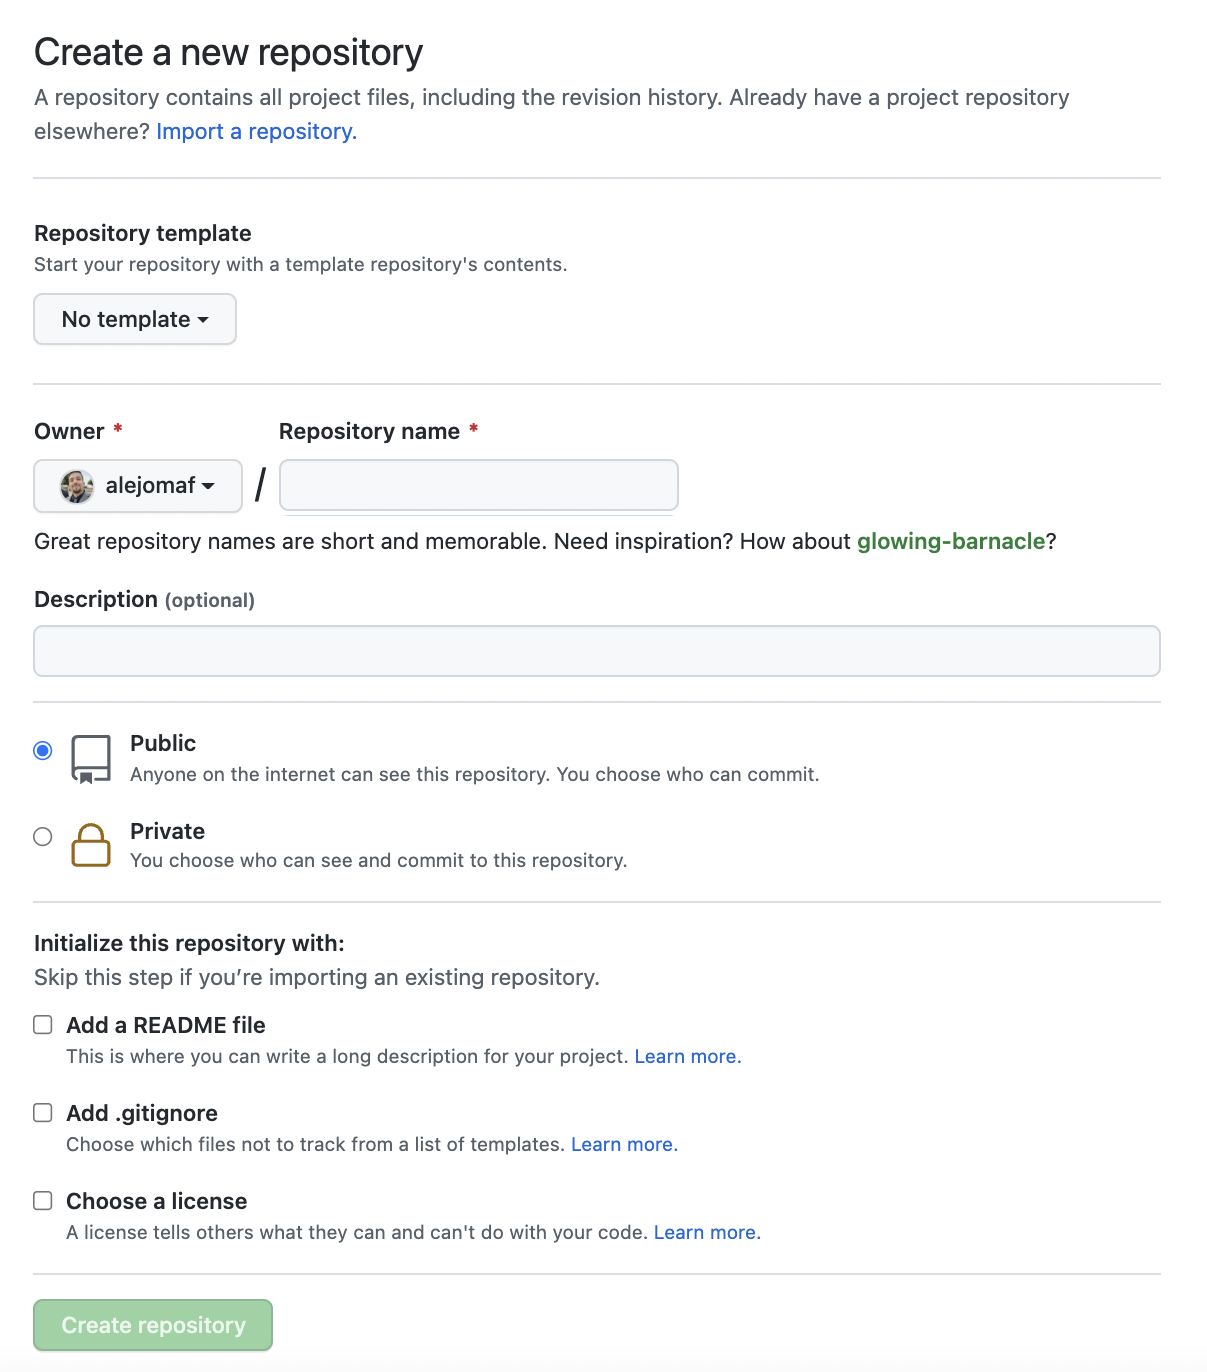
\includegraphics[scale=0.4]{preparacion_entorno/creando_nuevo_repositorio.png}
            \caption{Creando un nuevo repositorio dentro de GitHub}
    \end{figure}
\end{enumerate}

Con estos sencillos pasos ya tendríamos creado nuestro repositorio.

\subsection{Visual Studio Code y Google Cloud, los mejores amigos}
Hoy en día lo nuevo y a lo que nos dirigimos es la nube. Dentro de ella se pretenden que se realicen todos los procesos. La mayoría de herramientas y servicios que se nos ofrece hoy en día cumplen un modelo de caja negra. Es decir, interactuamos con él y recibimos respuestas pero no vemos qué procesos ocurren dentro de aquella cajita.
\\Por esta razón cada vez se empieza a disponer menos de un software como tal y se empiezan a pasar a servicios en línea. Esto no quiere decir que se dejen de usar programas o aplicaciones móviles. Pero la realidad es que sin internet; la mayoría no funcionaría.
\\Esto presenta desventajas siendo la principal que se depende constantemente de una conexión en línea que puede parecer que pasa en todos sitios pero en lugares remotos lejos de la ciudad como son los pueblos de montaña el internet no es el mejor compañero por decirlo de una manera. Por suerte este no es mi caso.
\\Las ventajas son enormes aunque solo nos centraremos en las que para mí implican mayor relevancia.
\\El tener ya un repositorio generado con nuestro proyecto subido dentro de él ya nos aporta bastante autonomía ya que podemos acceder a él y descargar nuestros datos desde cualquier lugar. Pero, ¿y configurarlo?
\\Aquí viene una problemática que no nos resuelve un entorno de repositorios. El tener que configurarlo todo cada vez que queremos trabajar desde un sitio distinto. Esto nos lo resuelven las máquinas virtuales en la nube. El generar un directorio de trabajo donde poder conectar nuestro Visual Studio Code y olvidarnos de preocupaciones.
\\Lo segundo que me parece más importante es el ahorro de memoria tanto de RAM como de disco y de procesos que se origina al hacer esto. No es lo mismo tener que trabajar con un portátil conectado todo el día a un enchufe que poder ir llevándotelo contigo por el escaso consumo de su batería. Peor si es una torre, solo puedes trabajar desde un único sitio, con la problemática también de que siempre se te puede cortar la luz, y más en una zona de pueblo de sierra como es la mía, suele ocurrir una vez cada dos semanas.
\\Estas ventajas expuesta son las que personalmente me favorecen a mí, pero ¿y si trabajara con un equipo? El poder tener varios compañeros de un mismo equipo trabajando en el mismo proyecto, tocando los distintos componentes que se están desarrollando dentro de tu aplicación es fantástico.

\subsubsection{Crear una máquina virtual en Google Cloud}
